\begin{exercise}
      {ID-503c459c7d2f9e288382dfd3c75f6ab6ef46e733}
      {Lücken im Prozessdiagramm}
  \ifproblem\problem\par
    % <PROBLEM>
    Gegeben ist ein Prozessdiagramm, in dem einige
    Übergangswahrscheinlichkeiten fehlen.
    \begin{center}
      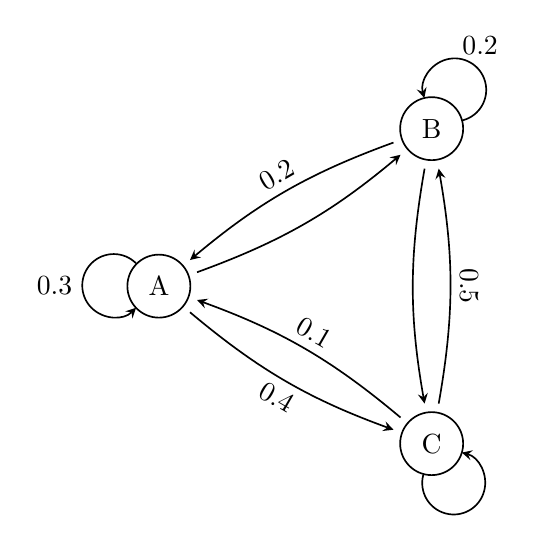
\begin{tikzpicture}[line width=0.6pt]
        \node[shape=circle, minimum size=8mm, inner sep=0pt, draw=black] (A) at (0, 0) {A};
        \node[shape=circle, minimum size=8mm, inner sep=0pt, draw=black] (B) at (30:4cm) {B};
        \node[shape=circle, minimum size=8mm, inner sep=0pt, draw=black] (C) at (330:4cm) {C};
        \begin{scope}[->, >=stealth, shorten <=3pt, shorten >=3pt]
          % A -- B
          \draw (A.20) to[out=20, in=220] node {} (B.220);
          \draw (B.200) to[out=200, in=40] node[rotate=30, above] {\num{0.2}} (A.40);
          % A -- C
          \draw (A.320) to[out=320, in=160] node[rotate=-30, below] {\num{0.4}} (C.160);
          \draw (C.140) to[out=140, in=340] node[rotate=-30, above] {\num{0.1}} (A.340);
          % B -- C
          \draw (B.260) to[out=260, in=100] (C.100);
          \draw (C.80) to[out=80, in=280] node[rotate=270, above] {\num{0.5}} (B.280);
        \end{scope}
        % A -- A
        \draw[->, >=stealth]
             (A.135)
              arc[start angle=45,
                  end angle=315,
                  radius=4mm]
              node[pos=0.5, shift={(180:10pt)}] {\num{0.3}};
        % B -- B
        \draw[->, >=stealth]
             (B.15)
              arc[start angle=285,
                  end angle=555,
                  radius=4mm]
              node[pos=0.5, shift={(60:7pt)}] {\num{0.2}};
        % C -- C
        \draw[->, >=stealth]
             (C.255)
              arc[start angle=165,
                  end angle=435,
                  radius=4mm];
      \end{tikzpicture}
    \end{center}
    \begin{enumerate}[a)]
      \item Berechnen und ergänzen Sie die fehlenden
            Übergangswahrscheinlichkeiten im oberen
            Prozessdiagramm.
      \item Bestimmen Sie die Übergangsmatrix für das
            vollständige Prozessdiagramm.
      \item Zu Beginn befinden sich \num{100} Personen
            in Zustand A und je \num{200} Personen in
            Zustand B und C.
            Berechnen Sie wie viele Personen sich in den
            Zuständen nach einem Übergang und nach
            fünf Übergängen befinden.
    \end{enumerate}
    % </PROBLEM>
  \fi
  %\ifoutline\outline\par
    % <OUTLINE>
    % </OUTLINE>
  %\fi
  %\ifoutcome\outcome\par
    % <OUTCOME>
    % </OUTCOME>
  %\fi
\end{exercise}
